\documentclass{beamer}

% to include graphics
\usepackage{graphicx}

% to include hyperlinks
\usepackage{hyperref}

% divide slides into columns
\usepackage{multicol}


\usetheme{Copenhagen}
\usecolortheme{beaver}

\title{Cluster Progress}
\date{\today}

\begin{document}

%----------BEGIN TITLE----------

\begin{frame}
  \maketitle
\end{frame}

%-----------END TITLE-----------

%----------BEGIN NAS-0----------

\begin{frame}
  \frametitle{NAS-0 and NAS-1 Drive Replacement}

  \begin{itemize}    
  \item The three faulted drives in NAS-0 have been replaced successfully! All drives are now online.
  \item One drive failed in NAS-1, and it was replaced successfully as well.
    % we have 3 more 2TB spares upstairs (nas1)
    % (two?) of the 750GB drives were fixed and can be reused (nas0)
  \end{itemize}

  \begin{figure}[H]
    \begin{center}
      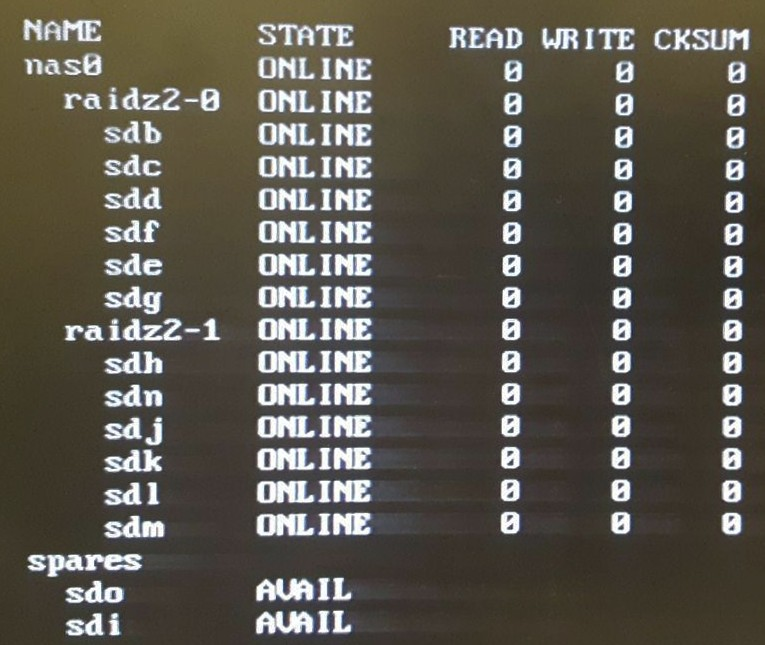
\includegraphics[width=0.5\textwidth]{nas0_drives_good.jpg}
    \end{center}
  \end{figure}

\end{frame}

%-----------END NAS-0-----------
%-----------BEGIN HDFS----------
\begin{frame}
  \frametitle{HDFS Installation}

  \begin{itemize}
  \item HDFS (Hadoop) has been installed on the SE.
    %with the SE as the "Primary Namenode"
    %figure out what, if any, is the secondary namenode
    %figure out what the DataNodes are - not the compute nodes, Datanodes store HDFS data. 
  \item It still needs to be configured, however.
    %Create users needed for grid operation and the respective areas
    %configure GridFTP - reads the Hadoop configuration file to learn how to talk to Hadoop
  \end{itemize}

  \begin{figure}[H]
    \begin{center}
      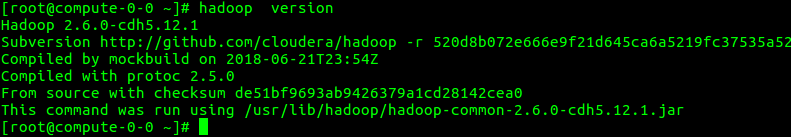
\includegraphics[width=0.9\textwidth]{hadoop_version.png}
    \end{center}
   \end{figure}
  
\end{frame}
%-----------END HDFS------------
\end{document}
